\documentclass{article}

\usepackage[english, russian]{babel}
\usepackage{geometry}
\usepackage{graphicx}
\usepackage{listings}
\usepackage{xcolor}
\usepackage[14pt]{extsizes}
\usepackage{amsmath}
\usepackage{setspace}
\usepackage{multirow}
\usepackage{tocloft}
\usepackage{indentfirst} 
\usepackage{lipsum}
\usepackage{caption}

\RequirePackage{cmap}
\RequirePackage[utf8]{inputenc}
\RequirePackage[T2A]{fontenc}
\captionsetup[figure]{name={Рисунок},labelsep=endash}
\captionsetup[table]{singlelinecheck=false, labelsep=endash}

\renewcommand{\cftsecleader}{\cftdotfill{\cftdotsep}}
\geometry{pdftex, left = 3cm, right = 1cm	, top = 2cm, bottom = 2cm}
\onehalfspacing

\setlength{\parindent}{1,25cm}
\lstdefinestyle{python}{
	language={Python},
	basicstyle=\footnotesize\ttfamily,
	frame=single,
	tabsize=4,	
	breaklines=true
}

\DeclareCaptionLabelSeparator{line}{\ --\ }
\DeclareCaptionFont{white}{\color{white}}
\DeclareCaptionFormat{listing}{\colorbox[cmyk]{0.43,0.35,0.35,0.01}{\parbox{\textwidth}{\hspace{15pt}#1#2#3}}}
\captionsetup[lstlisting]{
	labelsep=line
}

\begin{document}
\begin{titlepage}
	\newgeometry{pdftex, left=2cm, right=2cm, top=2.5cm, bottom=2.5cm}
	\fontsize{12pt}{12pt}\selectfont
	\noindent\begin{tabular}{|c|c|}	\hline
	\noindent\begin{minipage}{0.15\textwidth}
		
\includegraphics[width=\linewidth]{tools/logo.png}
	\end{minipage} &
	\noindent\begin{minipage}{0.85\textwidth}\centering
		\textbf{\newline Министерство науки и высшего образования Российской Федерации}\\
		\textbf{Федеральное государственное бюджетное образовательное учреждение высшего образования}\\
		\textbf{«Московский государственный технический университет имени Н.Э.~Баумана}\\
		\textbf{(национальный исследовательский университет)»}\\
		\textbf{(МГТУ им. Н.Э.~Баумана)}
	\end{minipage} \\
	\hline	\end{tabular}\newline\newline\newline
	\noindent ФАКУЛЬТЕТ \underline{«Информатика и системы управления»} \newline\newline
	\noindent КАФЕДРА \underline{«Программное обеспечение ЭВМ и информационные технологии»}\newline\newline\newline\newline\newline\newline

	\noindent\begin{minipage}{1.0\textwidth}\centering
		\Large\textbf{   ~~~ Лабораторная работа №3}\newline
		\textbf{по дисциплине «Анализ алгоритмов»}\newline\newline\newline\newline\newline
	\end{minipage}

	\noindent\textbf{Тема} \underline{Поиск элемента в массиве}\newline\newline
	\textbf{Студент} \underline{Тузов Даниил Александрович}\newline\newline
	\textbf{Группа} \underline{ИУ7-52Б}\newline\newline
	\textbf{Преподаватель} \underline{Кормановский Михаил Владимирович}
	
	\begin{center}
		\vfill
		Москва, \the\year ~г.
	\end{center}
	\restoregeometry
	\clearpage
\end{titlepage}

\renewcommand{\contentsname}{СОДЕРЖАНИЕ} 
\tableofcontents
\setcounter{page}{2}
\clearpage

\section*{ВВЕДЕНИЕ}
\addcontentsline{toc}{section}{ВВЕДЕНИЕ}
В третьей лабораторной работе по анализу алгоритмов рассматриваются алгоритмы поиска в массиве.

Целью лабораторной работы является изучение алгоритмов поиска элемента в массиве.
Для достижения поставленной цели небходимо решить следующие задачи:
\begin{itemize}
	\item изучить теоретические аспекты алгоритмов поиска в массиве;
	\item разработать алгоритмы поиска в массиве:
	\begin{itemize}
		\item алгоритм линейного поиска;
		\item алгоритм бинарного поиска;
	\end{itemize}
	\item провести для каждого алгоритма сравнительный анализ количества операций сравнения относительно 
	расположения искомого элемента в массиве;
	\item обосновать полученные результаты.
\end{itemize}


\clearpage\section{Аналитическая часть}
В этой части рассматриваются теоретические аспекты алгоритмов поиска в массиве.

\subsection{Линейный поиск}
Линейный поиск (также известный как последовательный поиск) -- это алгоритм поиска элемента в списке или массиве,
который последовательно проверяет каждый элемент до тех пор, пока не найдёт совпадение или не проверит все элементы.

Сложность такого алгоритма $O(N)^{[1]}$, где $N$ -- это размер массива, в котором ищется элемент. 

\subsection{Бинарный поиск}
Бинарный поиск -- это алгоритм поиска элемента в отсортированном массиве (векторе). Также известен как метод деления 
пополам или дихотомия.

Принцип работы бинарного поиска:
\begin{enumerate}
	\item определяется значение элемента в середине структуры данных;
	\item полученное значение сравнивается с ключом;
	\item если ключ меньше значения середины, то поиск осуществляется в первой половине элементов, иначе -- во второй;
	\item поиск сводится к тому, что вновь определяется значение серединного элемента в выбранной половине и 
сравнивается с ключом;
	\item процесс продолжается до тех пор, пока не будет найден элемент со значением ключа или не станет пустым интервал 
для поиска. 
\end{enumerate}

Сложность такого алгоритма $O(logN)^{[1]}$, где $N$ -- это размер массива, в котором ищется элемент. 

\subsection{Вывод}
В этой части были рассмотрены теоретические аспекты алгоритмов поиска в массиве: алгоритма линейного поиска и
алгоритмов бинарного поиска. Заявленная сложность алгоритма бинарного поиска лучше, чем у алгоритма линейного поиска.


\clearpage\section{Конструкторская часть}
В этой части представлены описания алгоритмов.

\subsection{Описание алгоритмов}
На вход алгоритмам подаются массив \texttt{arr} (для бинарного поиска массив отсортирован) и искомый элемент \texttt{el}, на 
выходе единственное число -- индекс элемента в массиве или значение -1, если элемент не найден.

На рисунках \ref{scheme:LP} - \ref{scheme:BP} приведены описания алгоритмов.
	
\begin{figure}[h]
	\centering
	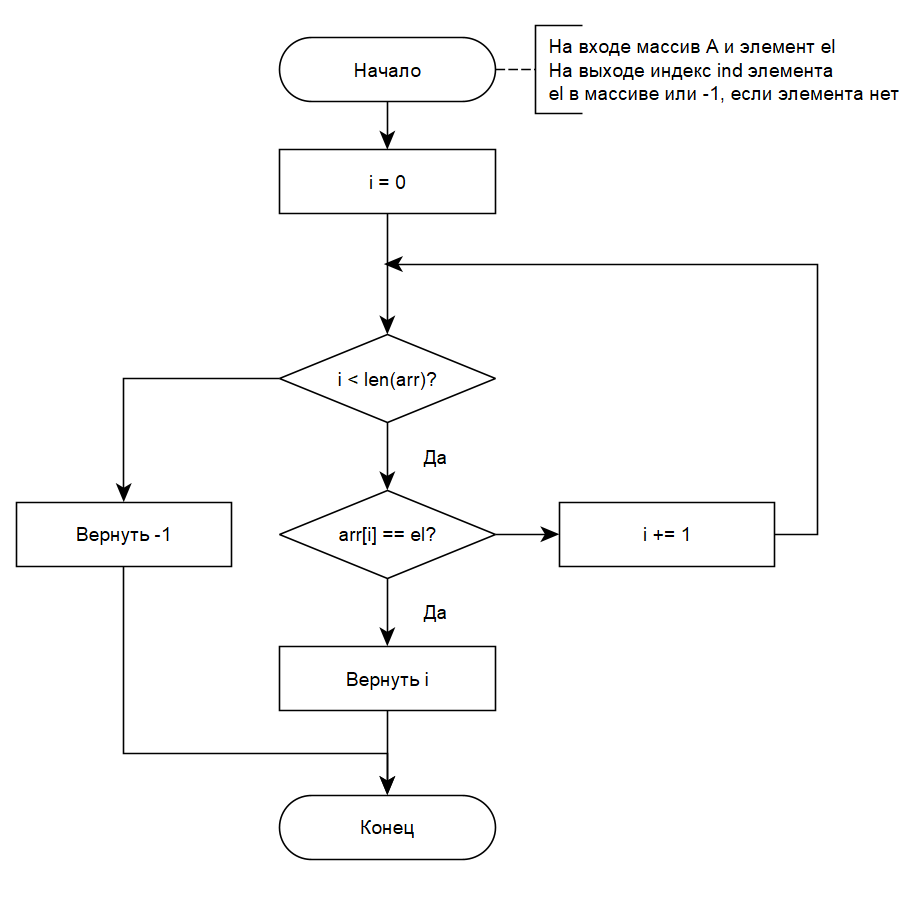
\includegraphics[scale=0.8]{tools/alg_1.png}
	\caption{Описание алгоритма линейного поиска в массиве}
	\label{scheme:LP}
\end{figure}

\begin{figure}[h]
	\centering
	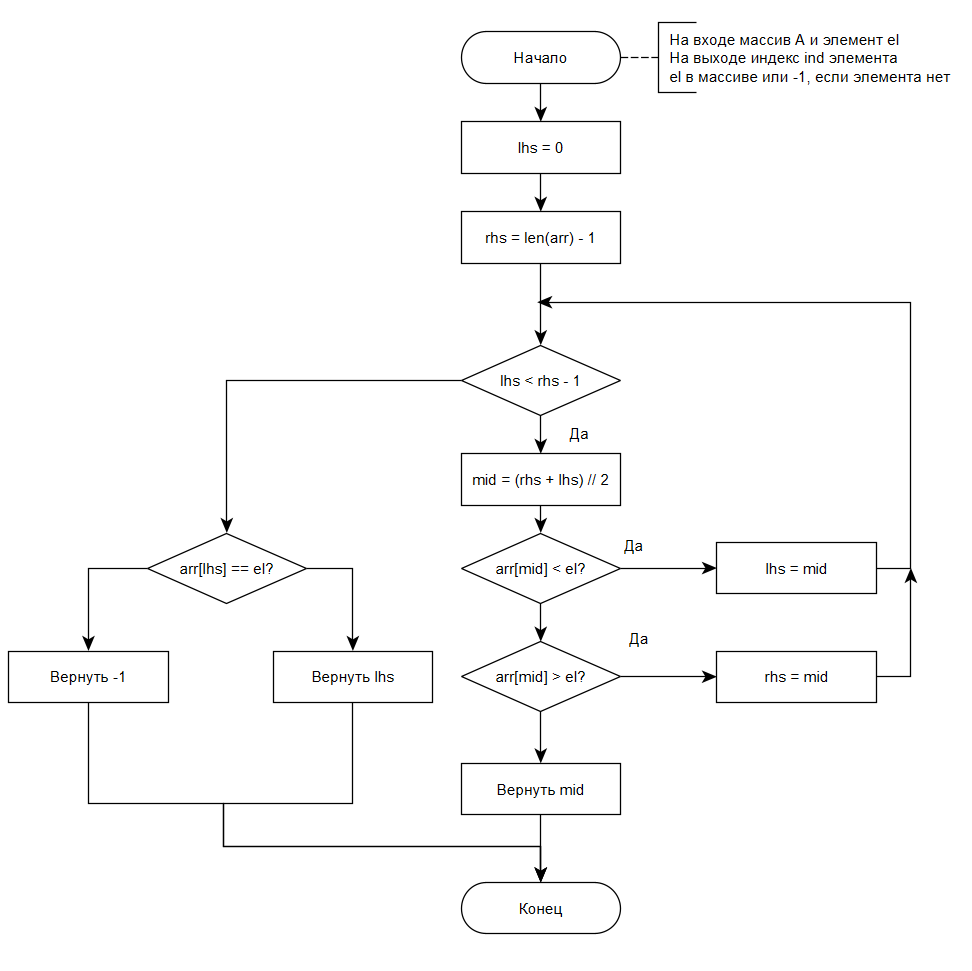
\includegraphics[scale=0.85]{tools/alg_2.png}
	\caption{Описание алгоритма бинарного поиска в массиве}
	\label{scheme:BP}
\end{figure}

\clearpage\subsection{Вывод}
В этом разделе на основе теоретических аспектов были представлены описания алгоритма линейного поиска в массиве
и алгоритма бинарного поиска в массиве.


\clearpage\section{Технологическая часть}
В этом разделе обоснованы средства реализации, а так же представлены реализации алгоритмов и функциональные тесты.

\subsection{Средства реализации}
Для реализации алгоритмов в этой лабораторной работы был выбран язык $Python^{[2]}$, потому что в нем нет 
автоматического сборщика мусора.

\subsection{Реализация алгоритмов}
В листингах \ref{lst:LP} - \ref{lst:BP} представлены коды написанных алгоритмов.

\begin{lstlisting}[style=python, label=lst:LP,caption=Алгоритм линейного поиска в массиве]
def linear_search(arr, x):
    if len(arr) == 0:
        return -1, 0

    compares = 0
    for ind, i in enumerate(arr):
        compares += 1
        if i == x:
            return ind + 1, compares

    return -1, compares
\end{lstlisting}

\clearpage\begin{lstlisting}[style=python, label=lst:BP,caption=Алгоритм бинарного поиска в массиве]
def binary_search(arr, x):
    if len(arr) == 0:
        return -1, 0

    compares = 0
    lhs = 0
    rhs = len(arr)
    while lhs < rhs - 1:
        compares += 1
        mid = (rhs + lhs) // 2
        if arr[mid] == x:
            return mid + 1, compares
        elif arr[mid] < x:
            lhs = mid
        else:
            rhs = mid

    compares += 1
    if arr[lhs] != x:
        return -1, compares

    return lhs + 1, compares
\end{lstlisting}

\clearpage\subsection{Функциональные тесты}
В таблице \ref{tbl:func_test} приведены функциональные тесты, на которых тестировалась программа.
\begin{table}[h]
	\begin{center}
	\caption{\label{tbl:func_test} Функциональные тесты, на которых были протестированы алгоритмы}
	\begin{tabular}{|c|c|c|c|}
		\hline
		Массив & Искомый элемент & Линейный поиск &  Бинарный поиск
		\\ \hline
		[ ] & 1 & -1 & -1  
		\\ \hline
		[ 1 ] & 2 & -1 & -1                             
		\\ \hline
		[ 1, 2, 3, 4, 5 ] & 0 & -1 & -1 
		\\ \hline
		[ 1, 2, 3, 4, 5 ] & 1 & 1 & 1 
		\\ \hline
		[ 1, 2, 3, 4, 5 ] & 2 & 2 & 2 
		\\ \hline
		[ 1, 2, 3, 4, 5 ] & 3 & 3 & 3 
		\\ \hline
		[ 1, 2, 3, 4, 5 ] & 4 & 4 & 4 
		\\ \hline
		[ 1, 2, 3, 4, 5 ] & 5 & 5 & 5 
		\\ \hline
		[ 1, 2, 3, 4, 5 ] & 6 & -1 & -1 
		\\ \hline
		[ 1, 2, 3, 4 ] & 4 & 4 & 4 
		\\ \hline
		[ 1, 2, 3, 4 ] & 1 & 1 & 1 
		\\ \hline
		[ 1, 2, 3, 4 ] & 0 & -1 & -1 
		\\ \hline
	\end{tabular}
	\end{center}
\end{table}

\subsection{Вывод}
В этом разделе на основе описаний алгоритмов были написаны и представлены коды алгоритмов. Помимо кодов
представлены функциональные тесты, на которых был протестирован каждый алгоритм. Причем функциональные тесты
обеспечивают полное покрытие кода$^{[5]}$.


\clearpage\section{Исследовательская часть}
В этом разделе приведен сравнительный анализ алгоритмов по количеству операций сравнения, необходимых для того, чтобы 
найти искомый элемент в массиве.

\subsection{Технические характеристики ЭВМ}
Все замеры проводились на ЭВМ, характеристики которой приведены ниже:
\begin{itemize}
	\item Процессор -- 12th Gen Intel(R) Core(TM) i5-12450H   2.00 ГГц
	\item Оперативная память -- 16,0 ГБ
	\item Тип системы -- 64-разрядная операционная система, процессор x64
	\item Операционная система -- Windows 11
	\item Версия ОС -- 23H2
\end{itemize}

\subsection{Сравнение алгоритмов}
Размер массива, на котором проводилось исследование равен 1028. Предварительно массив был заполнен случайным образом
с помощью библиотеки $random^{[3]}$. Графики построены с помощью библиотеки $matplotlib^{[4]}$. На рисунках  \ref{grph:LP} 
- \ref{grph:BP} представлена зависимость количества сравнений от расположения искомого элемента для алгоритмов линейного 
и бинарного поиска. На рисунке \ref{grph:BP_sort} приведена отсортированная гистограмма из рисунка \ref{grph:BP}.

\begin{figure}[h]
	\centering
	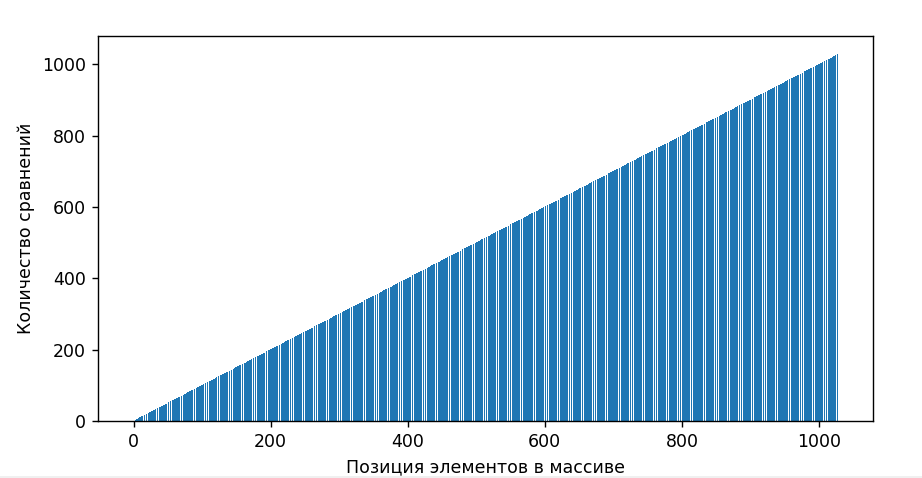
\includegraphics[scale=0.9]{tools/Screenshot_1.png}
	\caption{Алгоритм линейного поиска}
	\label{grph:LP}
\end{figure}

\begin{figure}[h]
	\centering
	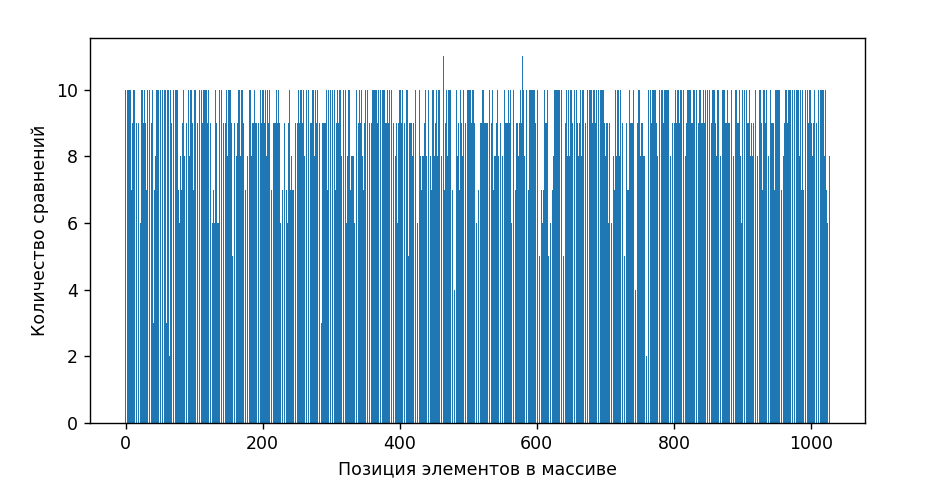
\includegraphics[scale=0.9]{tools/Screenshot_2.png}
	\caption{Алгоритм бинарного поиска}
	\label{grph:BP}
\end{figure}

\begin{figure}[h]
	\centering
	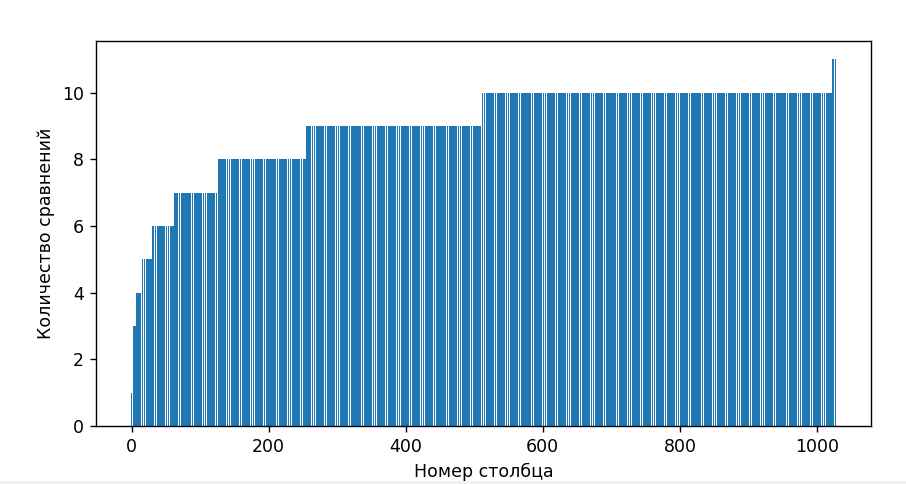
\includegraphics[scale=0.9]{tools/Screenshot_3.png}
	\caption{Алгоритм бинарного поиска с сортировкой значений гистограммы}
	\label{grph:BP_sort}
\end{figure}

\clearpage\subsection{Вывод}
В этом разделе приведен сравнительный анализ алгоритмов. Исследована зависимость количества сравнений, необходимых, 
чтобы найти элемент в массиве, от расположения элемента в массиве. Оказалось, что в линейном алгоритме количество
сравнений изменяется прямопропорционально индексу расположения элемента в массиве. Так же линейный поиск
проигрывает бинарному поиску в количестве операций сравнения. Из рисунка \ref{grph:BP_sort} видно, что количество
операций сравнений не превышает величину равную логарифму от размера массива.


\clearpage\section*{ЗАКЛЮЧЕНИЕ}
\addcontentsline{toc}{section}{ЗАКЛЮЧЕНИЕ}
В ходе выполнения лабораторной работы поставленная цель была достигнута, а также были решены следующие задачи:
\begin{itemize}
	\item изучены теоретические аспекты алгоритмов поиска в массиве;
	\item реализованы алгоритмы на языке $Python$; 
	\item проведено сравнение алгоритмов по количеству операций сравнения, необходимых для того, чтобы найти
	искомый элемент в массиве:
	\begin{itemize}
		\item в алгоритме с линейным поиском эта величина прямопропорциональна индексу искомого элемента в массиве;
		\item количество операций сравнения меньше в бинарном поиске;
		\item количество операций сравнения не превышает логарифма от размера массива;
	\end{itemize}
	\item описаны и обоснованы полученные результаты.
\end{itemize} 

\clearpage\section*{СПИСОК ИСПОЛЬЗОВАННЫХ ИСТОЧНИКОВ}
\addcontentsline{toc}{section}{СПИСОК ИСПОЛЬЗОВАННЫХ ИСТОЧНИКОВ}
\begin{enumerate}
	\item Никлаус Вирт Алгоритмы и структуры данных. Новая версия для Оберона. Никлаус Вирт. — М.: ДМК Пресс, 2016 — 272 c.
	\item Welcome to Python -- https://www.python.org
	\item	Библиотека random -- https://docs.python.org/3/library/random.html
	\item	Библиотека matplotlib -- https://matplotlib.org/
	\item Утилита coverage -- https://coverage.readthedocs.io/en/latest/
\end{enumerate}

\end{document}